\section{Rete neurale ricorrente}
\subsection{Numero di input}
Teoricamente ad una RNN basterebbe una sola nota in input per imparare una canzone intera, visto che ha memoria di quello che ha visto ed in che ordine lo ha visto, della storia passata, ma si \`e reso necessario ampliare l'input ad $N$\footnote{Il numero di note in input viene definito appropriatamente in ogni esperimento;} note (come viene fatto in~\cite{todd1989}) perch\`e una sola non risultava sufficiente per limiti di hardware.
Con pi\`u note si usano cone input la probabilit\`a che la rete indovini il target aumenta perch\`e rendiamo esplicita un pezzo di storia della canzone (le $N$ note precedenti al target).
Durante la fase di scrittura del codice \`e stata riscontrata una relazione tra il numero di note in input e la correttezza dell'output che conferma quanto detto; ovvero se come input si dava una sequenza composta solo da una sola nota questa riusciva a predirne correttamente solo un'altra come successiva. Se quindi ci si trovava nella situazione di una doppia scelta ecco che la rete non riusciva pi\`u a distinguere le due note.
Sempre facendo riferimento allo scritto citato sopra~\cite{todd1989} si legge che la rete creata era caratterizzata dall'avere otto note come input. Non c'\`e un modo per decidere arbitrariamente il numero di note in input ma bisogna trovare un compromesso tra la quantit\`a di sequenze che si possono riconoscere e la complessit\`a del sistema.

\subsection{Tipo di rete utilizzata}
La rete neurale ricorrente \`e cos\`i composta:
\begin{itemize}
\item[-]1 layer di input con $Nnote*11$ neuroni;
\item[-]1 hidden layer con $x$ neuroni\footnote{Il numero esatto di neuroni presenti nell'hidden layer viene definito appropriatamente in ogni esperimento;};
\item[-]1 layer di output con 11 neuroni.
\end{itemize}
C'\`e una full connection tra il layer di input e l'hidden layer, tra l'hidden layer e il layer di output e tra l'hidden layer e se stesso. \footnote{I pesi che portano dal nodo $A$ al nodo $B$ possono essere diversi di quelli che portano dal nodo $B$ al nodo $A$;}
La rete neurale non ricorrente \`e identica solo non presenta la connessione tra l'hidden layer e se stesso.\\
Le funzioni utilizzate all'interno dei neuroni sono di due tipi:
\begin{itemize}
\item[-] Sigmoidale;
\item[-] Long Short Term Memory (LSTM).
\end{itemize}
Un neurone di tipo LSTM \`e un neurone che ricorda i valori per un determinato periodo mentre uno sigmoidale implementa una funzione simile a quella sottostante.

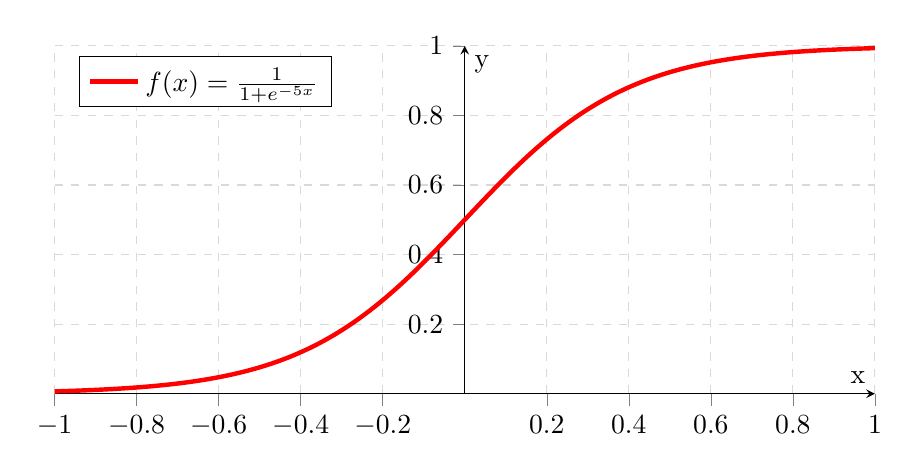
\begin{tikzpicture}
    \begin{axis}[
    	legend pos=north west,
        axis x line=middle,
        axis y line=middle,
        grid = major,
        width=12cm,
        height=6cm,
        grid style={dashed, gray!30},
        xmin=-1,     % start the diagram at this x-coordinate
        xmax= 1,    % end   the diagram at this x-coordinate
        ymin= 0,     % start the diagram at this y-coordinate
        ymax= 1,   % end   the diagram at this y-coordinate
        %axis background/.style={fill=white},
        xlabel=x,
        ylabel=y,
        tick align=outside,
        enlargelimits=false]
      % plot the stirling-formulae
      \addplot[domain=-1:1, red, ultra thick,samples=500] {1/(1+exp(-5*x))}; 
      \addlegendentry{$f(x)=\frac{1}{1+e^{-5x}}$}
    \end{axis} 
\end{tikzpicture}

A seconda del tipo di rete utilizzata cambiano i tipi di neuroni (per esempio quelli LSTM possono essere utilizzati solo con RNN). Quelli utilizzati nel programma sono:\\
\begin{table}[ht]
\centering
\begin{tabular}{| c | c | c |}
\multicolumn {3}{c}{\textbf{Tipi di neurone}}\\
\hline
&\textbf{FFN}&\textbf{RNN}\\\hline
Hidden Neuron&Sigmoidal&LSTM\\\hline
Output Neuron&Sigmoidal&Sigmoidal\\\hline
\end{tabular}
\end{table}
\\\\\\
Il seguente grafo rappresenta la RNN, con la connessione ricorrente trai i neuroni presenti nell'hidden layer.\\
\input{graph}